% Social Media and the Virtues
% Chapter 2: Computing and AI Ethics
% Brendan Shea, PhD
% Rochester Community and Technical College

\documentclass[aspectratio=169]{beamer}

% References
\usepackage[backend=biber,style=authoryear]{biblatex}
\addbibresource{refs.bib}

% Theme and colors
\usetheme{Madrid}
\usecolortheme{whale}
\setbeamertemplate{navigation symbols}{}
\setbeamertemplate{footline}[frame number]

% Packages
\usepackage[utf8]{inputenc}
\usepackage[T1]{fontenc}
\usepackage{graphicx}
\usepackage{booktabs}
\usepackage{array}
\usepackage{multirow}
\usepackage{csquotes}

% TikZ and libraries
\usepackage{tikz}
\usetikzlibrary{shapes.geometric, arrows.meta, positioning, calc, backgrounds, fit, decorations.pathreplacing, shadows, mindmap, trees, shapes.symbols}

\definecolor{primaryblue}{RGB}{0,74,124}
\definecolor{accentorange}{RGB}{230,126,34}
\definecolor{lightgray}{RGB}{245,245,245}
\definecolor{darktext}{RGB}{44,62,80}
\definecolor{virtuegreen}{RGB}{39,174,96}
\definecolor{viceред}{RGB}{192,57,43}
\definecolor{socialblue}{RGB}{29,161,242}

% Custom TikZ styles for virtue ethics diagrams
\tikzset{
    virtue/.style={rectangle, rounded corners, draw=virtuegreen, fill=virtuegreen!20, thick, minimum width=2.5cm, minimum height=0.8cm, font=\small},
    vice/.style={rectangle, rounded corners, draw=viceред, fill=viceред!20, thick, minimum width=2.5cm, minimum height=0.8cm, font=\small},
    concept/.style={rectangle, rounded corners, draw=primaryblue, fill=primaryblue!15, thick, minimum width=2.5cm, minimum height=0.8cm, font=\small},
    platform/.style={rectangle, rounded corners, draw=socialblue, fill=socialblue!15, thick, minimum width=2cm, minimum height=0.7cm, font=\footnotesize},
    timeline/.style={->, thick, primaryblue},
    arrow/.style={-{Stealth[length=3mm]}, thick, primaryblue},
}

% Title information
\title[Social Media \& Virtues]{Social Media and the Virtues}
\subtitle{Chapter 2: Computing and AI Ethics}
\author{Brendan Shea, PhD}
\institute[RCTC]{Rochester Community and Technical College}
\date{}

\usepackage{lmodern}

\begin{document}

% ============================================
% SLIDE 1: Title Slide
% ============================================
\begin{frame}
    \titlepage
    \begin{center}
        
\begin{tikzpicture}
            \node[concept, minimum width=4cm] (ancient) at (-3,0) {Ancient Wisdom};
            \node[concept, minimum width=4cm] (modern) at (3,0) {Digital Age};
            \draw[arrow, <->] (ancient) -- (modern);
        \end{tikzpicture}
    \end{center}
\end{frame}

% ============================================
% SLIDE 2: Essential Questions
% ============================================
\begin{frame}{Essential Questions}
    \begin{itemize}
        \item What kind of people do we \textbf{become} through our daily digital habits and social media use?
        \item Can \textbf{virtue ethics}---a 2,400-year-old philosophical tradition---help us navigate the challenges of social media?
        \item How has the rise of \textbf{Web 2.0} fundamentally changed the way we form communities and relationships?
        \item Is social media actually causing a \textbf{mental health crisis} among teenagers, or is the evidence more complicated?
    \end{itemize}
    
    \begin{alertblock}{Guiding Theme}
        ``We are what we repeatedly do. Excellence, then, is not an act, but a habit.'' ---Aristotle
    \end{alertblock}
\end{frame}

% ============================================
% SLIDE 3: Why Virtue Ethics for Social Media?
% ============================================
\begin{frame}{Why Virtue Ethics for Social Media?}
    \begin{itemize}
        \item \textbf{Rule-based ethics} asks: ``Is this particular action right or wrong?''
        \item \textbf{Virtue ethics} asks: ``What kind of person does this action make me over time?''
        \item Social media is not just about individual posts or clicks---it \textbf{shapes our character} through daily habits.
        \item Philosopher Shannon Vallor argues that technologies can either \textbf{cultivate or undermine} virtues like patience, honesty, and empathy.
    \end{itemize}
    
    \begin{block}{Key Insight}
        Virtue ethics focuses on long-term character formation, making it especially suited for analyzing technologies we use every day.
    \end{block}
\end{frame}

% ============================================
% SLIDE 4: Aristotle and Eudaimonia
% ============================================
\begin{frame}{Aristotle and Eudaimonia}
    \begin{columns}[T]
        \begin{column}{0.6\textwidth}
            \begin{itemize}
                \item \textbf{Aristotle (384--322 BCE)} was a Greek philosopher, student of Plato, and tutor to Alexander the Great.
                \item \textbf{Eudaimonia} is often translated as ``happiness,'' but is better understood as ``human flourishing'' or ``living well.'' (\cite{aristotle_nicomachean})
                \item Eudaimonia is not a temporary feeling but a \textbf{way of living}---achieving your full potential as a human being.
                \item Aristotle's key insight: ``Happiness is an activity of the soul in accordance with \textbf{virtue}.''
            \end{itemize}
        \end{column}
        \begin{column}{0.35\textwidth}
            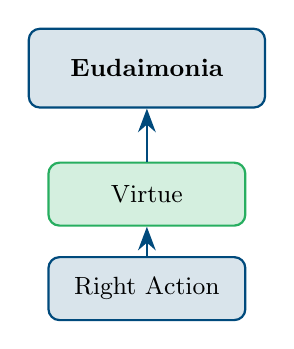
\begin{tikzpicture}[scale=0.8]
                \node[concept, minimum width=3cm, minimum height=1cm] (eud) at (0,2) {\textbf{Eudaimonia}};
                \node[virtue, minimum width=2.5cm] (virtue) at (0,0) {Virtue};
                \node[concept, minimum width=2.5cm] (action) at (0,-1.5) {Right Action};
                \draw[arrow] (virtue) -- (eud);
                \draw[arrow] (action) -- (virtue);
            \end{tikzpicture}
        \end{column}
    \end{columns}
\end{frame}

% Social Media and the Virtues - Slides 5-8
% Insert after slide 4 in main document

% ============================================
% SLIDE 5: What Are the Virtues?
% ============================================
\begin{frame}{What Are the Virtues?}
    \begin{itemize}
        \item A \textbf{virtue} is a stable character trait that enables us to act well and to flourish as human beings.
        \item Virtues are developed through \textbf{practice and habituation}---we become courageous by repeatedly acting courageously.
        \item Each virtue lies between two corresponding \textbf{vices}: one of excess and one of deficiency.
    \end{itemize}
    
    \vspace{0.3cm}
    \begin{table}[h]
        \centering
        \small
        \begin{tabular}{>{\raggedright}p{2.5cm} >{\centering}p{2.5cm} >{\raggedleft\arraybackslash}p{2.5cm}}
            \toprule
            \textbf{Vice (Deficiency)} & \textbf{Virtue (Mean)} & \textbf{Vice (Excess)} \\
            \midrule
            Cowardice & Courage & Recklessness \\
            Insensibility & Temperance & Self-indulgence \\
            Stinginess & Generosity & Wastefulness \\
            Self-deprecation & Truthfulness & Boastfulness \\
            \bottomrule
        \end{tabular}
    \end{table}
\end{frame}

% ============================================
% SLIDE 6: The Doctrine of the Mean
% ============================================
\begin{frame}{The Doctrine of the Mean}
    \begin{itemize}
        \item \textbf{The doctrine of the mean} states that virtue is the balanced midpoint between two extremes (vices of excess and deficiency).
        \item The mean is \textbf{not mathematical}---it varies depending on the person, situation, and context.
        \item Finding the mean requires \textbf{practical wisdom} (phronesis) to judge what is appropriate in each circumstance.
    \end{itemize}
    
    \begin{center}
        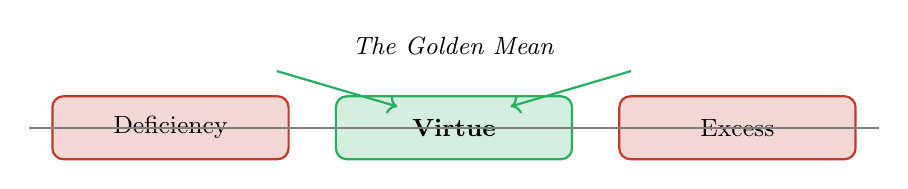
\begin{tikzpicture}[scale=0.9]
            \node[vice, minimum width=3cm] (def) at (-4,0) {Deficiency};
            \node[virtue, minimum width=3cm] (virt) at (0,0) {\textbf{Virtue}};
            \node[vice, minimum width=3cm] (exc) at (4,0) {Excess};
            \draw[thick, gray] (-6,0) -- (6,0);
            \draw[thick, virtuegreen, ->] (-2.5,0.8) -- (-0.8,0.3);
            \draw[thick, virtuegreen, ->] (2.5,0.8) -- (0.8,0.3);
            \node[above] at (0,0.9) {\small \textit{The Golden Mean}};
        \end{tikzpicture}
    \end{center}
\end{frame}

% ============================================
% SLIDE 7: Phronesis---Practical Wisdom
% ============================================
\begin{frame}{Phronesis---Practical Wisdom}
    \begin{itemize}
        \item \textbf{Phronesis} (practical wisdom) is the intellectual virtue of knowing what to do in particular situations.
        \item It is not enough to know \textit{that} honesty is good---phronesis tells us \textit{how} to be honest in a specific context.
        \item Susan Sauvé Meyer: ``You are not a good person unless you exercise \textbf{good judgment}.''
        \item Phronesis is developed through \textbf{experience and reflection}, not just by learning abstract rules.
    \end{itemize}
    
    \begin{exampleblock}{Applying Phronesis to Social Media}
        Practical wisdom helps us judge: When should I post? What should I share? How should I respond to criticism? What content deserves my attention?
    \end{exampleblock}
\end{frame}

% ============================================
% SLIDE 8: Aristotelian Virtues for Social Media
% ============================================
\begin{frame}{Aristotelian Virtues for Social Media}
    \begin{itemize}
        \item \textbf{Truthfulness online}: Are you presenting yourself honestly, or does your profile show a more glamorous life than reality?
        \item \textbf{Appropriate humor}: Aristotle recognized that jokes often come at someone's expense---what will you laugh at or share?
        \item \textbf{Self-presentation}: The vice of excess is \textbf{bragging}; the vice of deficiency is \textbf{false modesty} or inauthenticity.
    \end{itemize}
    
    \begin{block}{Key Insight from Susan Sauvé Meyer (\cite{meyer_aristotelian_virtues})}
        Technology has increased our opportunities for social interaction, but it has not changed our fundamental human concern with how others perceive us.
    \end{block}
\end{frame}

% Social Media and the Virtues - Slides 9-12
% Insert after slide 8 in main document

% Social Media and the Virtues - Slides 9-12 (REVISED v2)
% Strengthened focus on civic virtue and democratic citizenship

% ============================================
% SLIDE 9: Communitarianism and Civic Virtue
% ============================================
\begin{frame}{Communitarianism and Civic Virtue}
    \begin{itemize}
        \item \textbf{Communitarianism} emphasizes that human identity and virtue are formed within communities---including \textbf{political communities}.
        \item Key thinkers (MacIntyre, Sandel, Taylor) argue that liberal individualism neglects our obligations to the \textbf{common good}.
        \item \textbf{Civic virtues} are character traits necessary for democratic citizenship: tolerance, civic friendship, commitment to truth, willingness to deliberate.
        \item Aristotle: Humans are \textit{zoon politikon}---``political animals'' who flourish through participation in \textbf{shared civic life}.
    \end{itemize}
    
    \begin{block}{Michael Sandel on Civic Virtue}
        Democracy requires more than voting---it requires citizens with the \textbf{character} to engage respectfully with those who disagree, to seek common ground, and to place the common good above narrow self-interest. (\cite{sandel_democracy})
    \end{block}
\end{frame}

% ============================================
% SLIDE 10: The Civic Virtues in Detail
% ============================================
\begin{frame}{The Civic Virtues in Detail}
    \begin{columns}[T]
        \begin{column}{0.48\textwidth}
            \textbf{Essential Civic Virtues:}
            \begin{itemize}
                \item \textbf{Civic friendship}: Seeing political opponents as fellow citizens, not enemies
                \item \textbf{Tolerance}: Respecting others' right to hold different views
                \item \textbf{Deliberative capacity}: Ability to reason together about the common good
            \end{itemize}
        \end{column}
        \begin{column}{0.48\textwidth}
            \textbf{Supporting Virtues:}
            \begin{itemize}
                \item \textbf{Epistemic humility}: Acknowledging we might be wrong
                \item \textbf{Commitment to truth}: Valuing facts over tribal loyalty
                \item \textbf{Civility}: Engaging respectfully even in disagreement
            \end{itemize}
        \end{column}
    \end{columns}
    
    \vspace{0.3cm}
    \begin{alertblock}{The Democratic Stakes}
        These virtues aren't optional extras---they're \textbf{necessary conditions} for democracy to function. Without them, we get tribalism, gridlock, and the erosion of shared reality.
    \end{alertblock}
\end{frame}

% ============================================
% SLIDE 11: MacIntyre, Practices, and the Common Good
% ============================================
\begin{frame}{MacIntyre, Practices, and the Common Good}
    \begin{itemize}
        \item Alasdair MacIntyre's \textit{After Virtue} (\cite{macintyre_after_virtue}) warned that modern society has lost \textbf{shared frameworks} for moral reasoning.
        \item Without shared traditions and practices, moral discourse becomes mere assertion of preferences---``emotivism.''
        \item \textbf{Key insight}: Virtues are cultivated through participation in \textbf{practices} with shared standards and goods.
        \item Democratic deliberation is itself a \textbf{practice} requiring specific virtues: listening, reasoning, compromising.
    \end{itemize}
    
    \begin{exampleblock}{The Question for Our Age}
        If virtues require shared practices and communities, what happens when our primary ``community'' is a social media feed algorithmically designed to show us only what we already believe?
    \end{exampleblock}
\end{frame}

% ============================================
% SLIDE 12: Review Questions---Part 1
% ============================================
\begin{frame}{Review Questions---Part 1}
    \begin{enumerate}
        \item \textbf{Define eudaimonia.} Why is ``flourishing'' considered a better translation than simply ``happiness''?
        
        \vspace{0.15cm}
        \item \textbf{Explain the doctrine of the mean} using an example relevant to social media use.
        
        \vspace{0.15cm}
        \item \textbf{What are ``civic virtues''?} Why do communitarians believe they are essential for democracy?
        
        \vspace{0.15cm}
        \item \textbf{According to MacIntyre,} what has modern society ``lost'' that makes moral reasoning difficult? How might this apply to online discourse?
        
        \vspace{0.15cm}
        \item \textbf{Discussion}: Can a person develop civic virtues like tolerance and deliberative capacity primarily through online political engagement? Why or why not?
    \end{enumerate}
\end{frame}

% ============================================
% SLIDE 13: Part 2 Introduction---Technology and the Virtues
% ============================================
\begin{frame}{Technology and the Virtues}
    \begin{itemize}
        \item Recall: For Aristotle, virtues are developed through \textbf{practice within communities} that model and reinforce good character.
        \item Philosopher \textbf{Shannon Vallor} argues that technologies are not neutral tools---they \textbf{shape the conditions} under which virtues can (or cannot) flourish. (\cite{vallor_technology_virtues})
        \item \textbf{Key question for Part 2}: How has the rise of Web 2.0 changed the communities and practices through which we develop virtue?
        \item Psychologist \textbf{Sherry Turkle} warns that digital communication may undermine capacities for empathy, patience, and authentic self-knowledge.
    \end{itemize}
    
    \begin{alertblock}{Vallor's Central Claim}
        ``New social media invite \textbf{new habits} of communication and social interaction... [that] have the potential to impact our cultivation of the virtues.'' ---Shannon Vallor, \textit{Technology and the Virtues} (2016)
    \end{alertblock}
\end{frame}

% ============================================
% SLIDE 14: Before Web 2.0---Communities of Virtue
% ============================================
\begin{frame}{Before Web 2.0---Communities of Virtue}
    \begin{itemize}
        \item \textbf{Web 1.0} (approximately 1991--2004) was the ``read-only'' web---users consumed content created by professionals.
        \item From a virtue ethics perspective, Web 1.0 had \textbf{limited impact} on character formation---it was more like a library than a community.
        \item Traditional \textbf{communities of practice} (families, schools, neighborhoods, churches) remained the primary sites where virtues were cultivated.
        \item Face-to-face interaction was still the default mode of social life, preserving opportunities for \textbf{empathy, patience, and presence}.
    \end{itemize}
    
    \begin{block}{Aristotle's Insight}
        Virtue is formed through repeated practice in community with others who model good character. The question: What happens when our ``communities'' become digital?
    \end{block}
\end{frame}

% ============================================
% SLIDE 15: Defining Web 2.0---A New Context for Character
% ============================================
\begin{frame}{Defining Web 2.0---A New Context for Character}
    \begin{itemize}
        \item \textbf{``Web 2.0''} (coined 1999, popularized 2004) marked the shift from passive consumption to active participation online.
        \item Tim O'Reilly's definition: ``The web as a platform''---users now \textbf{create content}, not just consume it.
        \item From a virtue perspective, this is profound: our daily \textbf{habits of communication and self-presentation} now occur in digital spaces.
        \item Vallor asks: Do these new habits cultivate virtues like honesty and empathy---or do they cultivate their opposing vices?
    \end{itemize}
    
    \begin{exampleblock}{The Virtue Ethics Question}
        Web 2.0 isn't just a technological change---it's a change in the \textbf{environment where character is formed}. What kind of people are we becoming through our daily digital practices?
    \end{exampleblock}
\end{frame}

% ============================================
% SLIDE 16: Core Characteristics Through a Virtue Lens
% ============================================
\begin{frame}{Core Characteristics Through a Virtue Lens}
    \begin{columns}[T]
        \begin{column}{0.48\textwidth}
            \textbf{Web 2.0 Features:}
            \begin{itemize}
                \item User-generated content
                \item Social networking
                \item Participation and collaboration
                \item Global reach and scale
            \end{itemize}
        \end{column}
        \begin{column}{0.48\textwidth}
            \textbf{Virtue Implications:}
            \begin{itemize}
                \item New contexts for \textbf{truthfulness} (or deception)
                \item New forms of \textbf{friendship} (or isolation)
                \item Opportunities for \textbf{generosity}---or narcissism
                \item \textbf{Weak ties} replace thick community
            \end{itemize}
        \end{column}
    \end{columns}
    
    \vspace{0.3cm}
    \begin{alertblock}{Sherry Turkle's Warning}
        ``We expect more from technology and less from each other.'' Digital connection may \textbf{simulate} community without providing the sustained, embodied relationships where virtue actually develops. (\cite{turkle_alone_together})  
    \end{alertblock}
\end{frame}

% Social Media and the Virtues - Slides 17-20 (REVISED)
% PART 2 continued: With virtue ethics as analytical lens

% ============================================
% SLIDE 17: TIME Person of the Year 2006---Optimism and Concern
% ============================================
\begin{frame}{TIME Person of the Year 2006---Optimism and Concern}
    \begin{itemize}
        \item In 2006, \textbf{TIME Magazine} named ``You'' as Person of the Year, celebrating user-generated content and collaboration. (\cite{time_you_2006})
        \item TIME declared: ``It's about the many wresting power from the few and helping one another for nothing.''
        \item From a virtue perspective, this \textbf{optimistic vision} emphasized potential for generosity, collaboration, and democratic participation.
        \item But even then, some worried: Would online interaction cultivate \textbf{genuine virtue}---or merely its appearance?
    \end{itemize}
    
    \begin{block}{The Aristotelian Question}
        Aristotle distinguished between \textbf{true virtue} (stable character expressed consistently) and merely \textbf{appearing virtuous} in particular situations. Does social media reward genuine character---or performative displays?
    \end{block}
\end{frame}

% ============================================
% SLIDE 18: Platform Evolution and Habit Formation
% ============================================
\begin{frame}{Platform Evolution and Habit Formation}
    \begin{center}
        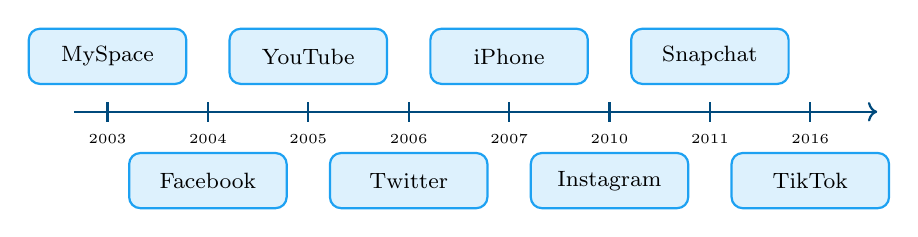
\begin{tikzpicture}[scale=0.85]
            \draw[thick, primaryblue, ->] (0,0) -- (12,0);
            \foreach \x/\year in {0.5/2003, 2/2004, 3.5/2005, 5/2006, 6.5/2007, 8/2010, 9.5/2011, 11/2016} {
                \draw[thick, primaryblue] (\x,-0.15) -- (\x,0.15);
                \node[below, font=\tiny] at (\x,-0.2) {\year};
            }
            \node[platform, above] at (0.5,0.4) {MySpace};
            \node[platform, below] at (2,-0.6) {Facebook};
            \node[platform, above] at (3.5,0.4) {YouTube};
            \node[platform, below] at (5,-0.6) {Twitter};
            \node[platform, above] at (6.5,0.4) {iPhone};
            \node[platform, below] at (8,-0.6) {Instagram};
            \node[platform, above] at (9.5,0.4) {Snapchat};
            \node[platform, below] at (11,-0.6) {TikTok};
        \end{tikzpicture}
    \end{center}
    
    \vspace{0.2cm}
    \begin{itemize}
        \item Each platform introduced new \textbf{habits of interaction}: status updates, likes, stories, short videos.
        \item Recall Aristotle: ``We are what we repeatedly do.'' These daily micro-habits \textbf{shape character over time}.
        \item Vallor notes that platforms are designed to maximize engagement---not to cultivate user flourishing.
    \end{itemize}
\end{frame}

% ============================================
% SLIDE 19: The Smartphone and Constant Connectivity
% ============================================
\begin{frame}{The Smartphone and Constant Connectivity}
    \begin{itemize}
        \item The \textbf{iPhone} (2007) put social media in our pockets, enabling constant connectivity and instant response.
        \item Sherry Turkle argues this undermines \textbf{solitude}---the capacity to be alone with one's thoughts, essential for self-knowledge. 
        \item Constant notifications interrupt \textbf{sustained attention}---what Vallor calls a key ``technomoral virtue'' for our age.
        \item The virtue of \textbf{patience} is particularly challenged when we expect instant responses and infinite content.
    \end{itemize}
    
    \begin{alertblock}{Turkle on Solitude and Self-Knowledge}
        ``If we don't teach our children to be alone, they will only know how to be \textbf{lonely}.'' Solitude is necessary for the self-reflection that virtue ethics requires.
    \end{alertblock}
\end{frame}

% ============================================
% SLIDE 20: Algorithms and the Erosion of Phronesis
% ============================================
\begin{frame}{Algorithms and the Erosion of Phronesis}
    \begin{itemize}
        \item \textbf{Algorithmic feeds} decide what we see based on predicted engagement---removing our need to \textit{choose} what deserves attention.
        \item This may erode \textbf{phronesis} (practical wisdom): the capacity to judge what is worth our time and attention.
        \item Content that triggers strong emotions (outrage, envy, fear) is amplified---potentially cultivating \textbf{vice} rather than virtue.
        \item Vallor warns of ``\textbf{moral deskilling}'': when technology makes choices for us, we lose practice in making them ourselves.
    \end{itemize}
    
    \begin{center}
        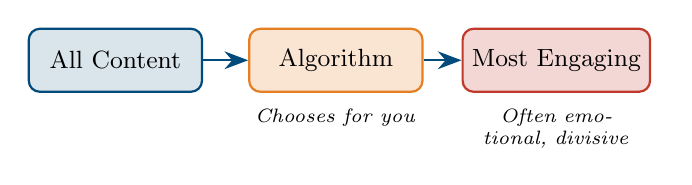
\begin{tikzpicture}[scale=0.7]
            \node[concept, minimum width=2.2cm] (all) at (0,0) {All Content};
            \node[concept, fill=accentorange!20, draw=accentorange, minimum width=2.2cm] (algo) at (4,0) {Algorithm};
            \node[vice, minimum width=2.2cm] (engage) at (8,0) {Most Engaging};
            \draw[arrow] (all) -- (algo);
            \draw[arrow] (algo) -- (engage);
            \node[below, font=\scriptsize] at (4,-0.7) {\textit{Chooses for you}};
            \node[below, font=\scriptsize, text width=2.5cm, align=center] at (8,-0.7) {\textit{Often emotional, divisive}};
        \end{tikzpicture}
    \end{center}
\end{frame}


% ============================================
% SLIDE 19: Echo Chambers and the Erosion of Civic Virtue
% ============================================
\begin{frame}{Echo Chambers and the Erosion of Civic Virtue}
    \begin{itemize}
        \item \textbf{Echo chambers} are social media environments where users encounter only views similar to their own.
        \item Algorithms maximize engagement by showing content that \textbf{confirms existing beliefs}---and outrage at the ``other side.''
        \item This directly undermines \textbf{civic virtues}: Why practice tolerance if you never encounter reasonable disagreement?
        \item Legal scholar Cass Sunstein warned in \textit{Republic.com} (2001) that personalized media would fragment the \textbf{shared public sphere} democracy requires.
    \end{itemize}
    
    \begin{alertblock}{The Filter Bubble Problem}
        Eli Pariser: Algorithms create ``\textbf{filter bubbles}'' that invisibly edit our view of the world. We lose the \textbf{common ground} necessary for democratic deliberation. (\cite{pariser_filter_bubble})
    \end{alertblock}
\end{frame}

% ============================================
% SLIDE 20: Polarization and the Decline of Civic Friendship
% ============================================
\begin{frame}{Polarization and the Decline of Civic Friendship}
    \begin{itemize}
        \item Research shows Americans have become significantly more \textbf{politically polarized} since the rise of social media.
        \item \textbf{Affective polarization}: We don't just disagree with the other party---we \textit{dislike} and \textit{distrust} them as people.
        \item This represents a failure of \textbf{civic friendship}---the Aristotelian virtue of seeing fellow citizens as partners in a shared project.
        \item Social media rewards \textbf{performative outrage} over thoughtful deliberation---cultivating vice, not virtue.
    \end{itemize}
    
    \begin{block}{Evidence of Polarization}
        Pew Research: The share of Americans with ``very unfavorable'' views of the opposing party has \textbf{more than doubled} since the 1990s. We increasingly see opponents as not just wrong, but as \textbf{threats to the nation}. (\cite{pew_teens_2024})
    \end{block}
\end{frame}


% Social Media and the Virtues - Slides 21-24 (REVISED v2)
% Part 2 conclusion with integrated civic virtue themes

% ============================================
% SLIDE 21: The Attention Economy and Democratic Attention
% ============================================
\begin{frame}{The Attention Economy and Democratic Attention}
    \begin{itemize}
        \item The \textbf{attention economy} captures our attention for profit---but attention is also a \textbf{civic resource}.
        \item Democracy requires citizens who can sustain attention on \textbf{complex issues}---not just react to outrage.
        \item Persuasive design (infinite scroll, notifications, variable rewards) trains us toward \textbf{distraction}, not deliberation.
        \item Platforms optimize for \textbf{engagement}, which favors emotional, divisive content over nuanced civic discourse.
    \end{itemize}
    
    \begin{block}{The Civic Cost of Distraction}
        Self-governance requires the capacity to \textbf{think carefully} about policy, weigh evidence, and consider long-term consequences. An attention economy that fragments focus undermines democratic competence itself.
    \end{block}
\end{frame}

% ============================================
% SLIDE 22: Turkle on Conversation, Empathy, and Citizenship
% ============================================
\begin{frame}{Turkle on Conversation, Empathy, and Citizenship}
    \begin{itemize}
        \item Sherry Turkle argues that \textbf{face-to-face conversation} is essential for developing empathy---a virtue with civic dimensions.
        \item \textbf{Civic empathy}: The capacity to understand fellow citizens' perspectives, even when we disagree.
        \item Digital communication lets us \textbf{curate and control}---we avoid the difficult work of truly listening to different views.
        \item Turkle: ``We expect more from technology and less from each other''---including less from ourselves as citizens.
    \end{itemize}
    
    \begin{alertblock}{Research Finding}
        One study suggests empathy among college students has \textbf{declined 40\%} since 2000. This affects not just personal relationships but our capacity for democratic life with diverse others. (\cite{konrath_empathy_decline})
    \end{alertblock}
\end{frame}

% ============================================
% SLIDE 23: Vallor's Technomoral Virtues---Personal and Civic
% ============================================
\begin{frame}{Vallor's Technomoral Virtues---Personal and Civic}
    \begin{columns}[T]
        \begin{column}{0.48\textwidth}
            \textbf{Personal Technomoral Virtues:}
            \begin{itemize}
                \item \textbf{Self-control}: Resisting compulsive use
                \item \textbf{Honesty}: Authentic self-presentation
                \item \textbf{Humility}: Accurate self-knowledge
                \item \textbf{Patience}: Tolerating delays and difficulty
            \end{itemize}
        \end{column}
        \begin{column}{0.48\textwidth}
            \textbf{Civic Technomoral Virtues:}
            \begin{itemize}
                \item \textbf{Civility}: Respectful disagreement
                \item \textbf{Justice}: Fair treatment online
                \item \textbf{Empathy}: Understanding diverse others
                \item \textbf{Epistemic responsibility}: Commitment to truth
            \end{itemize}
        \end{column}
    \end{columns}
    
    \vspace{0.3cm}
    \begin{block}{Technomoral Wisdom}
        \textbf{Technomoral wisdom} is the master virtue: knowing how to live well \textit{with} technology---both as individuals and as citizens of a democratic society.
    \end{block}
\end{frame}

% ============================================
% SLIDE 24: Review Questions---Part 2
% ============================================
\begin{frame}{Review Questions---Part 2}
    \begin{enumerate}
        \item \textbf{According to Vallor,} how do new technologies affect the development of virtue? Why aren't technologies ``neutral tools''?
        
        \vspace{0.12cm}
        \item \textbf{What are ``echo chambers''?} How do they threaten civic virtues like tolerance and deliberative capacity?
        
        \vspace{0.12cm}
        \item \textbf{Explain ``moral deskilling.''} How might algorithmic feeds contribute to this problem for both personal and civic virtue?
        
        \vspace{0.12cm}
        \item \textbf{Why does Turkle} emphasize face-to-face conversation? What virtues does it cultivate that digital communication may not?
        
        \vspace{0.12cm}
        \item \textbf{Discussion}: Vallor proposes ``technomoral virtues'' for the digital age. Which do you think is most important for \textit{democratic citizenship}? Why?
    \end{enumerate}
\end{frame}



% Social Media and the Virtues - Slides 25-28 (REVISED)
% PART 3: Statistics Through a Virtue Ethics Lens

% ============================================
% SLIDE 25: Part 3 Introduction---What the Numbers Tell Us About Character
% ============================================
\begin{frame}{What the Numbers Tell Us About Character}
    \begin{itemize}
        \item Statistics on social media use aren't just about \textbf{time}---they reveal patterns of \textbf{habit formation}.
        \item Recall Aristotle: Virtues (and vices) are formed through repeated practice over time.
        \item \textbf{Key question}: What do these usage patterns suggest about the character traits being cultivated in young people?
        \item We'll examine the data through the lens of specific virtues: \textbf{temperance}, \textbf{patience}, \textbf{honesty}, \textbf{empathy}, and \textbf{practical wisdom}.
    \end{itemize}
    
    \begin{block}{The Virtue Ethics Approach to Data}
        Instead of asking only ``Is social media harmful?'' we ask: ``What kind of people are we becoming through these daily digital habits?''
    \end{block}
\end{frame}

% ============================================
% SLIDE 26: Usage Statistics and Temperance (Pew 2024)
% ============================================
\begin{frame}{Usage Statistics and Temperance (Pew 2024)}
    \begin{itemize}
        \item \textbf{95\%} of American teens have smartphone access; \textbf{46\%} report being online ``almost constantly.''
        \item Average daily social media use: \textbf{4.8 hours}---nearly one-third of waking hours.
        \item \textbf{45\%} of teens say they spend ``too much time'' on social media---suggesting awareness that temperance is lacking.
        \item 44\% have tried to cut back, indicating a \textbf{struggle for self-control} against habit and design.
    \end{itemize}
    
    \begin{alertblock}{The Temperance Problem}
        When nearly half of users \textit{themselves} believe they use too much, we see evidence that the virtue of \textbf{temperance} (moderation) is being systematically undermined by platform design.
    \end{alertblock}
\end{frame}

% ============================================
% SLIDE 27: Daily Habits and Character Formation
% ============================================
\begin{frame}{Daily Habits and Character Formation}
    \begin{columns}[T]
        \begin{column}{0.55\textwidth}
            \textbf{Daily Usage Rates:}
            \begin{itemize}
                \item YouTube: 73\% daily (15\% constant)
                \item TikTok: 58\% daily (17\% constant)
                \item Instagram: 50\% daily (12\% constant)
                \item Snapchat: 50\% daily
            \end{itemize}
            
            \vspace{0.2cm}
            \textbf{Aristotle's Principle:}
            \begin{itemize}
                \item ``We are what we \textbf{repeatedly} do.''
                \item Daily habits become ingrained character.
            \end{itemize}
        \end{column}
        \begin{column}{0.42\textwidth}
            \begin{block}{Habits Being Formed}
                \begin{itemize}
                    \item Checking for notifications
                    \item Scrolling without purpose
                    \item Seeking external validation
                    \item Comparing self to others
                    \item Responding immediately
                \end{itemize}
            \end{block}
        \end{column}
    \end{columns}
\end{frame}

% ============================================
% SLIDE 28: Global Patterns and "Problematic Use"
% ============================================
\begin{frame}{Global Patterns and ``Problematic Use''}
    \begin{itemize}
        \item The \textbf{WHO Europe} study (2024) found 11\% of adolescents show ``problematic social media use''---up from 7\% in 2018.
        \item ``Problematic use'' means struggling to \textbf{control} use despite negative consequences---a failure of temperance and self-control.
        \item Girls report higher rates (13\%) than boys (9\%), suggesting gendered patterns in how platforms affect character.
        \item 36\% report \textbf{constant contact} with friends online---blurring boundaries between self and social network.
    \end{itemize}
    
    \begin{exampleblock}{Virtue Ethics Interpretation}
        ``Problematic use'' is essentially what Aristotle would call a \textbf{vice of excess}---the failure to find the moderate mean in digital engagement. The rise from 7\% to 11\% suggests this vice is spreading.
    \end{exampleblock}
\end{frame}

% Social Media and the Virtues - Slides 29-32 (REVISED)
% PART 3 continued: Statistics Through a Virtue Ethics Lens

% ============================================
% SLIDE 29: Social Connection and the Virtue of Friendship
% ============================================
\begin{frame}{Social Connection and the Virtue of Friendship}
    \begin{columns}[T]
        \begin{column}{0.48\textwidth}
            \textbf{What Teens Report (Pew 2024):}
            \begin{itemize}
                \item 74\% feel more connected to friends' lives.
                \item 52\% feel supported through tough times (down from 67\% in 2022).
                \item Many cite community and belonging as benefits.
            \end{itemize}
        \end{column}
        \begin{column}{0.48\textwidth}
            \textbf{Aristotle on Friendship:}
            \begin{itemize}
                \item True friendship requires \textbf{shared life} (suzên)---spending real time together.
                \item Virtue friendships are based on mutual character development.
                \item Utility/pleasure friendships are shallower.
            \end{itemize}
        \end{column}
    \end{columns}
    
    \vspace{0.3cm}
    \begin{alertblock}{A Troubling Decline}
        The drop from 67\% to 52\% feeling supported suggests that social media connections may be becoming \textbf{less sustaining}---more like Aristotle's shallow friendships of utility than deep friendships of virtue.
    \end{alertblock}
\end{frame}

% ============================================
% SLIDE 30: Honesty, Self-Presentation, and Vice
% ============================================
\begin{frame}{Honesty, Self-Presentation, and Vice}
    \begin{itemize}
        \item Recall Susan Sauvé Meyer: Social media creates new contexts for the virtue of \textbf{truthfulness} and its opposing vices.
        \item The vice of excess is \textbf{boastfulness}---presenting a more glamorous life than reality (the ``highlight reel'' problem).
        \item The vice of deficiency is \textbf{false modesty} or \textbf{inauthenticity}---hiding one's true self entirely.
        \item 34\% of girls say social media makes them feel worse about their lives---evidence of harmful \textbf{social comparison} fueled by others' dishonest self-presentation.
    \end{itemize}
    
    \begin{block}{The Virtue of Truthfulness Online}
        The honest person presents themselves \textbf{accurately}---neither exaggerating accomplishments nor hiding genuine achievements. Social media's incentive structures make this mean \textit{very} difficult to hit.
    \end{block}
\end{frame}

% ============================================
% SLIDE 31: Sleep, Patience, and Self-Control
% ============================================
\begin{frame}{Sleep, Patience, and Self-Control}
    \begin{itemize}
        \item Research shows \textbf{nighttime social media use} is associated with poor sleep, anxiety, and depression (Woods \& Scott, 2016). (\cite{woods_scott_sleep})
        \item 36\% of teens maintain \textbf{constant online contact}---even at night when they should be resting.
        \item This reflects failures of \textbf{self-control} (the ability to resist immediate temptation) and \textbf{patience} (the ability to wait).
        \item Turkle: Constant connectivity prevents the \textbf{solitude} necessary for self-reflection and developing self-knowledge.
    \end{itemize}
    
    \begin{center}
        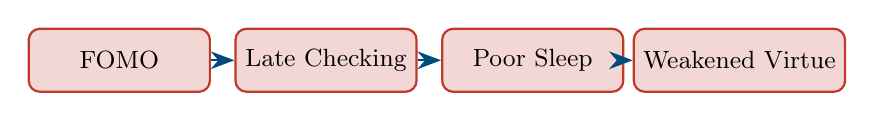
\begin{tikzpicture}[scale=0.75]
            \node[vice, minimum width=2.3cm] (fomo) at (0,0) {FOMO};
            \node[vice, minimum width=2.3cm] (check) at (3.5,0) {Late Checking};
            \node[vice, minimum width=2.3cm] (sleep) at (7,0) {Poor Sleep};
            \node[vice, minimum width=2.3cm] (virtue) at (10.5,0) {Weakened Virtue};
            \draw[arrow] (fomo) -- (check);
            \draw[arrow] (check) -- (sleep);
            \draw[arrow] (sleep) -- (virtue);
        \end{tikzpicture}
    \end{center}
\end{frame}

% ============================================
% SLIDE 32: Cyberbullying and the Failure of Civility
% ============================================
\begin{frame}{Cyberbullying and the Failure of Civility}
    \begin{itemize}
        \item Cyberbullying continues to rise among U.S. youth, representing a widespread \textbf{failure of the virtue of civility}.
        \item Vallor identifies \textbf{civility} as a key technomoral virtue: treating others with respect even in disagreement.
        \item Online environments may \textbf{disinhibit} vice: anonymity, distance, and lack of immediate feedback reduce natural restraints.
        \item The 24/7, permanent, public nature of online cruelty amplifies harm beyond traditional bullying.
    \end{itemize}
    
    \begin{exampleblock}{Why Digital Environments Challenge Civility}
        \begin{itemize}
            \item We don't see the \textbf{face} of the person we're hurting (reduced empathy cues)
            \item \textbf{Anonymity} removes accountability
            \item \textbf{Audience} rewards performative cruelty with engagement
            \item No opportunity for \textbf{repair} through face-to-face apology
        \end{itemize}
    \end{exampleblock}
\end{frame}

% Social Media and the Virtues - Slides 33-36 (REVISED)
% PART 3 concluded: Statistics Through a Virtue Ethics Lens

% ============================================
% SLIDE 33: Social Comparison and Humility
% ============================================
\begin{frame}{Social Comparison and Humility}
    \begin{itemize}
        \item \textbf{Social comparison} on platforms like Instagram and TikTok involves constantly measuring ourselves against others' curated images.
        \item This undermines \textbf{humility}---the virtue of accurate self-assessment, neither inflated nor deflated.
        \item 46\% of teens say social media makes them feel worse about their \textbf{body image}---evidence of distorted self-perception.
        \item The ``highlight reel'' effect: Comparing our ordinary reality to others' \textbf{best, edited moments}.
    \end{itemize}
    
    \begin{block}{Vallor on Humility as Technomoral Virtue}
        True humility means knowing our actual strengths and limitations. Constant exposure to idealized images makes this self-knowledge \textbf{systematically harder} to achieve.
    \end{block}
\end{frame}

% ============================================
% SLIDE 34: Positive Uses---When Does Social Media Cultivate Virtue?
% ============================================
\begin{frame}{When Does Social Media Cultivate Virtue?}
    \begin{itemize}
        \item Not all social media use undermines virtue---context and \textbf{manner of use} matter greatly.
        \item \textbf{Active use} (creating, meaningfully connecting) may cultivate virtues like creativity and genuine friendship.
        \item \textbf{Passive use} (scrolling, comparing) tends to cultivate vices like envy, impatience, and distorted self-image.
        \item Marginalized communities (LGBTQ+ youth, those with disabilities) may find \textbf{supportive communities} otherwise unavailable.
    \end{itemize}
    
    \begin{exampleblock}{Vallor's Key Distinction}
        Social media can \textbf{supplement} face-to-face relationships (potentially supporting virtue) or \textbf{substitute} for them (likely undermining virtue). The research suggests benefits come primarily from supplementation.
    \end{exampleblock}
\end{frame}

% ============================================
% SLIDE 35: The Challenge of Developing Phronesis
% ============================================
\begin{frame}{The Challenge of Developing Phronesis}
    \begin{itemize}
        \item \textbf{Phronesis} (practical wisdom) is the virtue of knowing how much, when, and in what way to engage with social media.
        \item Research struggles to identify a clear ``threshold''---suggesting the answer requires \textbf{individual judgment}, not universal rules.
        \item Orben \& Przybylski found small average effect sizes---but averages obscure the \textbf{individual differences} that phronesis must navigate. (\cite{orben_przybylski})
        \item The temperate mean will look different for different people in different circumstances.
    \end{itemize}
    
    \begin{alertblock}{Why Rules Aren't Enough}
        Virtue ethics recognizes that no simple rule (``2 hours max'') can replace the \textbf{practical wisdom} to judge what's appropriate for each person and situation. This is why character education matters more than screen-time limits.
    \end{alertblock}
\end{frame}

% ============================================
% SLIDE 36: Review Questions---Part 3
% ============================================
\begin{frame}{Review Questions---Part 3}
    \begin{enumerate}
        \item \textbf{How do usage statistics} reveal challenges to the virtue of \textbf{temperance}? What evidence suggests teens struggle with moderation?
        
        \vspace{0.15cm}
        \item \textbf{Explain the decline} from 67\% to 52\% in teens feeling supported. What does this suggest about online friendship from an Aristotelian perspective?
        
        \vspace{0.15cm}
        \item \textbf{How does social comparison} undermine the virtues of \textbf{truthfulness} (in those posting) and \textbf{humility} (in those viewing)?
        
        \vspace{0.15cm}
        \item \textbf{What is the difference} between active and passive social media use? Why might this distinction matter for virtue development?
        
        \vspace{0.15cm}
        \item \textbf{Discussion}: Why might simple screen-time rules be insufficient from a virtue ethics perspective? What role should \textbf{phronesis} play in managing social media use?
    \end{enumerate}
\end{frame}

% Social Media and the Virtues - Slides 37-40 (REVISED)
% PART 4: The Anxious Generation Debate Through a Virtue Lens

% ============================================
% SLIDE 37: Framing the Debate---Character and Resilience
% ============================================
\begin{frame}{Framing the Debate---Character and Resilience}
    \begin{itemize}
        \item Jonathan Haidt's \textit{The Anxious Generation} \parencite{haidt_anxious_generation} can be understood as a claim about \textbf{virtue formation}.
        \item His core argument: The ``phone-based childhood'' is producing young people who lack \textbf{resilience}---the ability to cope with adversity.
        \item Haidt draws on the concept of \textbf{antifragility}: like bones and muscles, character \textit{needs} challenges to develop strength.
        \item From a virtue ethics view, this is a claim that social media environments \textbf{systematically prevent} the development of certain virtues.
    \end{itemize}
    
    \begin{block}{The Virtue Ethics Translation}
        Haidt's thesis: Children are being denied the \textbf{practice and habituation} necessary to develop virtues like courage, resilience, and emotional regulation. Social media provides the wrong kind of challenges.
    \end{block}
\end{frame}

% ============================================
% SLIDE 38: Haidt's Evidence as Character Formation Data
% ============================================
\begin{frame}{Haidt's Evidence as Character Formation Data}
    \begin{itemize}
        \item \textbf{Timing} (decline begins ~2012): Coincides with smartphone saturation---a fundamental change in daily habits.
        \item \textbf{Gender patterns}: Girls, who use image-focused platforms more, show greater effects---consistent with virtue challenges around \textbf{truthfulness} and \textbf{humility}.
        \item \textbf{Multiple indicators}: Rising anxiety, depression, self-harm, and loneliness suggest failures in developing \textbf{emotional resilience}.
        \item Haidt frames this as a \textbf{generational character shift}---not individual pathology but systematic environmental change.
    \end{itemize}
    
    \begin{alertblock}{The Two-Part Problem (Virtue Ethics Reading)}
        \begin{enumerate}
            \item \textbf{Online}: Constant comparison, validation-seeking, and curated self-presentation cultivate \textit{vices}.
            \item \textbf{Offline}: ``Safetyism'' denies children the challenges needed to cultivate \textit{virtues} like courage and resilience.
        \end{enumerate}
    \end{alertblock}
\end{frame}

% ============================================
% SLIDE 39: The "Great Rewiring" as Habit Transformation
% ============================================
\begin{frame}{The ``Great Rewiring'' as Habit Transformation}
    \begin{columns}[T]
        \begin{column}{0.48\textwidth}
            \textbf{Play-Based Childhood Habits:}
            \begin{itemize}
                \item Negotiating conflicts face-to-face
                \item Tolerating boredom
                \item Taking physical risks
                \item Experiencing natural consequences
                \item Developing through unstructured play
            \end{itemize}
        \end{column}
        \begin{column}{0.48\textwidth}
            \textbf{Phone-Based Childhood Habits:}
            \begin{itemize}
                \item Avoiding difficult conversations
                \item Instant entertainment on demand
                \item Physical safety, digital exposure
                \item Algorithmically curated experience
                \item Constant adult monitoring
            \end{itemize}
        \end{column}
    \end{columns}
    
    \vspace{0.3cm}
    \begin{block}{Aristotle's Insight Applied}
        If ``we are what we repeatedly do,'' then these two childhoods are forming \textbf{fundamentally different characters}. Haidt argues the new habits cultivate fragility rather than resilience.
    \end{block}
\end{frame}

% ============================================
% SLIDE 40: Haidt's Recommendations as Virtue Interventions
% ============================================
\begin{frame}{Haidt's Recommendations as Virtue Interventions}
    \begin{enumerate}
        \item \textbf{No smartphones before high school}---Protect the period when foundational character habits are formed.
        \item \textbf{No social media before 16}---Delay exposure to environments that cultivate vices of comparison and validation-seeking.
        \item \textbf{Phone-free schools}---Restore opportunities for face-to-face interaction that cultivates empathy and social skills.
        \item \textbf{More unsupervised play}---Provide the challenges necessary to develop courage, resilience, and practical wisdom.
    \end{enumerate}
    
    \begin{exampleblock}{The Collective Action Argument}
        Individual families practicing these virtues face social costs. Haidt argues we need \textbf{community-wide norms}---precisely what communitarians like MacIntyre say virtue requires.
    \end{exampleblock}
\end{frame}

% Social Media and the Virtues - Slides 41-44 (REVISED)
% PART 4 continued: Critics and Responses Through a Virtue Lens

% ============================================
% SLIDE 41: The Critics---Questioning the Causal Story
% ============================================
\begin{frame}{The Critics---Questioning the Causal Story}
    \begin{itemize}
        \item \textbf{Candace Odgers} (\cite{odgers_anxious_review}) argues Haidt confuses correlation with causation.
        \item She points to alternative explanations: economic insecurity, school violence, climate anxiety, academic pressure.
        \item From a virtue perspective, these are \textit{also} challenges to character formation---but different ones than Haidt emphasizes.
        \item Critics argue the international patterns don't match smartphone adoption timing as closely as claimed.
    \end{itemize}
    
    \begin{block}{The Virtue of Intellectual Humility}
        Both sides of this debate should practice \textbf{intellectual humility}---acknowledging uncertainty, considering alternative views, and proportioning claims to evidence. This is itself a technomoral virtue.
    \end{block}
\end{frame}

% ============================================
% SLIDE 42: Research Quality and Epistemic Virtue
% ============================================
\begin{frame}{Research Quality and Epistemic Virtue}
    \begin{itemize}
        \item Critics like \textbf{Aaron Brown} \parencite*{brown_critique} and \textbf{Andrew Przybylski} argue that most studies Haidt cites have significant methodological weaknesses.
        \item Przybylski accuses Haidt of ``vote counting''---emphasizing \textbf{quantity} of studies over \textbf{quality} of evidence.
        \item Only 22 of 476 cited studies have data on \textit{both} heavy social media use \textit{and} serious mental health issues in adolescents.
        \item This raises questions about \textbf{epistemic virtues}: Are we believing what the evidence actually supports?
    \end{itemize}
    
    \begin{alertblock}{Vallor on Epistemic Virtue in a Digital Age}
        Vallor emphasizes that \textbf{good judgment about information} is a crucial technomoral virtue. The Haidt debate itself is a case study in how difficult this is when evidence is complex and stakes are high.
    \end{alertblock}
\end{frame}

% ============================================
% SLIDE 43: Alternative Explanations and Intellectual Honesty
% ============================================
\begin{frame}{Alternative Explanations and Intellectual Honesty}
    \begin{itemize}
        \item Critics suggest Haidt underweights alternative factors: economic precarity, academic pressure, COVID effects, climate anxiety.
        \item \textbf{Melinda Wenner Moyer}: ``I think Haidt is over-stating the research... in ways that undermine faith and trust in science.''
        \item \textbf{Tobias Dienlin}: The crisis may be ``largely limited to the U.S.''---suggesting cultural factors beyond technology.
        \item The virtue of \textbf{intellectual honesty} requires acknowledging what we don't know and presenting uncertainty accurately.
    \end{itemize}
    
    \begin{exampleblock}{Multiple Factors, One Framework}
        Even if social media is only \textit{one} factor among several, virtue ethics still provides a useful lens: All these challenges affect the \textbf{conditions under which character develops}. The question is which factors matter most.
    \end{exampleblock}
\end{frame}

% Social Media and the Virtues - Slides 45-48 (REVISED v2)
% Conclusion with integrated civic virtue themes

% ============================================
% SLIDE 45: The Full Picture---Personal and Civic Virtue
% ============================================
\begin{frame}{The Full Picture---Personal and Civic Virtue}
    \begin{itemize}
        \item Social media affects both \textbf{personal virtues} (temperance, patience, honesty) and \textbf{civic virtues} (tolerance, civic friendship, commitment to truth).
        \item Haidt focuses primarily on personal mental health; but the evidence also shows threats to \textbf{democratic health}.
        \item Echo chambers, polarization, and misinformation undermine the \textbf{shared civic life} communitarians say virtue requires.
        \item A complete analysis must address both individual flourishing \textit{and} our capacity for democratic self-governance.
    \end{itemize}
    
    \begin{block}{The Communitarian Synthesis}
        Personal and civic virtue are connected: We develop character \textit{within} communities, including political communities. When social media fragments the public sphere, it damages both individual and collective flourishing.
    \end{block}
\end{frame}

% ============================================
% SLIDE 46: Vallor, Turkle, and Democratic Renewal
% ============================================
\begin{frame}{Vallor, Turkle, and Democratic Renewal}
    \begin{columns}[T]
        \begin{column}{0.48\textwidth}
            \textbf{For Personal Virtue:}
            \begin{itemize}
                \item Cultivate \textbf{technomoral virtues}: temperance, honesty, patience, humility
                \item Reclaim \textbf{solitude} for self-reflection (Turkle)
                \item Practice \textbf{face-to-face} conversation
                \item Develop \textbf{technomoral wisdom} about personal use
            \end{itemize}
        \end{column}
        \begin{column}{0.48\textwidth}
            \textbf{For Civic Virtue:}
            \begin{itemize}
                \item Seek out \textbf{diverse viewpoints} intentionally
                \item Practice \textbf{epistemic humility} about political beliefs
                \item Cultivate \textbf{civic friendship} across divides
                \item Support \textbf{shared institutions} and factual discourse
            \end{itemize}
        \end{column}
    \end{columns}
    
    \vspace{0.3cm}
    \begin{alertblock}{The Dual Challenge}
        We need practices that cultivate both kinds of virtue---and we need \textbf{communities} (families, schools, civic organizations) that support these practices against algorithmic incentives.
    \end{alertblock}
\end{frame}

% ============================================
% SLIDE 47: Practical Wisdom for Personal and Civic Life
% ============================================
\begin{frame}{Practical Wisdom for Personal and Civic Life}
    \textbf{Questions for Personal Phronesis:}
    \begin{itemize}
        \item Am I practicing \textbf{temperance} in my social media use?
        \item Am I presenting myself with \textbf{truthfulness}, or curating a false image?
        \item Is my use \textbf{supplementing} or \textbf{substituting} for real relationships?
    \end{itemize}
    
    \vspace{0.2cm}
    \textbf{Questions for Civic Phronesis:}
    \begin{itemize}
        \item Do I encounter \textbf{diverse perspectives}, or only views I already hold?
        \item Do I treat political opponents as \textbf{fellow citizens} or as enemies?
        \item Am I committed to \textbf{truth} even when it challenges my beliefs?
        \item Am I contributing to \textbf{deliberation} or just performative outrage?
    \end{itemize}
    
    \begin{block}{Aristotle's Fundamental Question}
        ``What kind of \textbf{person}---and what kind of \textbf{citizen}---am I becoming through these daily digital habits?''
    \end{block}
\end{frame}

% ============================================
% SLIDE 48: Final Review Questions
% ============================================
\begin{frame}{Final Review Questions}
    \begin{enumerate}
        \item \textbf{Distinguish personal virtues from civic virtues.} How does social media potentially threaten each type?
        
        \vspace{0.1cm}
        \item \textbf{What is ``civic friendship''?} Why do communitarians believe it is essential for democracy, and how might social media undermine it?
        
        \vspace{0.1cm}
        \item \textbf{Explain the connection} between echo chambers, polarization, and the decline of deliberative capacity.
        
        \vspace{0.1cm}
        \item \textbf{Evaluate this claim}: ``The threat social media poses to democracy is more serious than its threat to individual mental health.'' Do you agree? Why or why not?
        
        \vspace{0.1cm}
        \item \textbf{Final Discussion}: Design a ``virtue-centered'' social media policy for a democratic society. What would it aim to cultivate? What practices and institutions would support it?
    \end{enumerate}
    
    \vspace{0.15cm}
    \textbf{Reflection}: What civic virtue do you most need to develop in your own online political engagement?
\end{frame}

\begin{frame}[allowframebreaks]{References}
    \printbibliography
\end{frame}


\end{document}